%! Suppress = MissingImport
%TODO: dodać screeny testów i krótkie opisy
\subsection{Testy modułu}\label{subsec:module-tests}
\begin{figure}[h]
    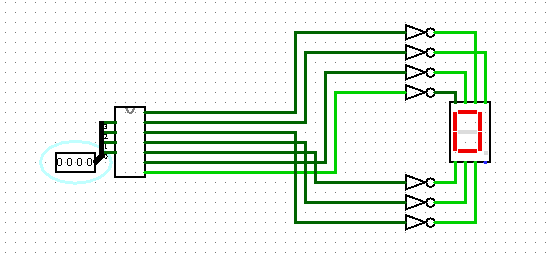
\includegraphics[width=\linewidth]{logisim_screenshots/0.png}
    \caption{Test 1}
    \label{fig:test0}
\end{figure}
Wejście (binarnie) 0000, oczekiwane wyjście (dziesiętnie) 0.\newline
Test 1 zakończony pomyślnie.

\begin{figure}[H]
    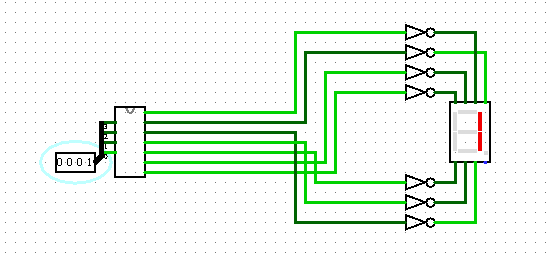
\includegraphics[width=\linewidth]{logisim_screenshots/1.png}
    \caption{Test 2}
    \label{fig:test1}
\end{figure}
Wejście (binarnie) 0001, oczekiwane wyjście (dziesiętnie) 1.\newline
Test 2 zakończony pomyślnie.

\begin{figure}[H]
    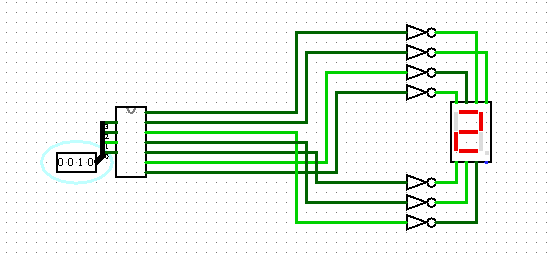
\includegraphics[width=\linewidth]{logisim_screenshots/2.png}
    \caption{Test 3}
    \label{fig:test2}
\end{figure}
Wejście (binarnie) 0010, oczekiwane wyjście (dziesiętnie) 2.\newline
Test 3 zakończony pomyślnie.

\begin{figure}[H]
    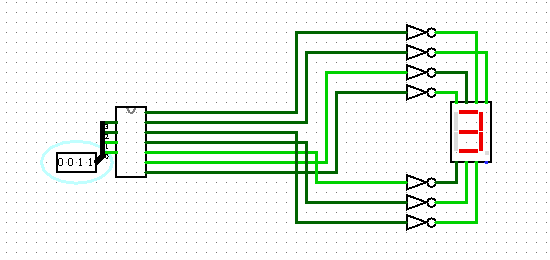
\includegraphics[width=\linewidth]{logisim_screenshots/3.png}
    \caption{Test 4}
    \label{fig:test3}
\end{figure}
Wejście (binarnie) 0011, oczekiwane wyjście (dziesiętnie) 3.\newline
Test 4 zakończony pomyślnie.

\begin{figure}[H]
    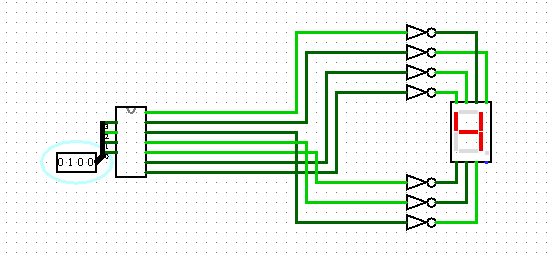
\includegraphics[width=\linewidth]{logisim_screenshots/4.png}
    \caption{Test 5}
    \label{fig:test4}
\end{figure}
Wejście (binarnie) 0100, oczekiwane wyjście (dziesiętnie) 4.\newline
Test 5 zakończony pomyślnie.

\begin{figure}[H]
    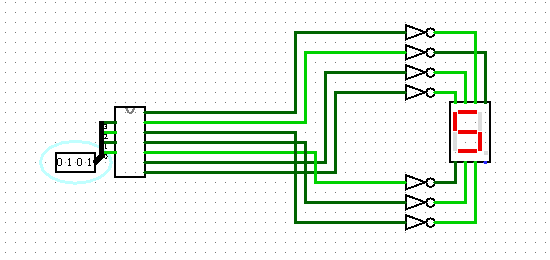
\includegraphics[width=\linewidth]{logisim_screenshots/5.png}
    \caption{Test 6}
    \label{fig:test5}
\end{figure}
Wejście (binarnie) 0101, oczekiwane wyjście (dziesiętnie) 5.\newline
Test 6 zakończony pomyślnie.

\begin{figure}[H]
    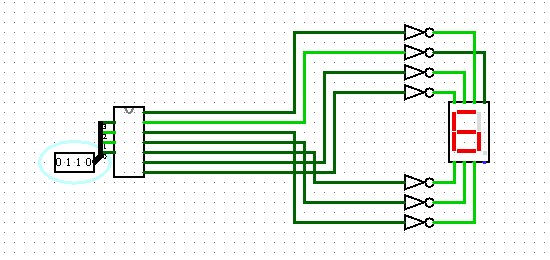
\includegraphics[width=\linewidth]{logisim_screenshots/6.png}
    \caption{Test 7}
    \label{fig:test6}
\end{figure}
Wejście (binarnie) 0110, oczekiwane wyjście (dziesiętnie) 6.\newline
Test 7 zakończony pomyślnie.

\begin{figure}[H]
    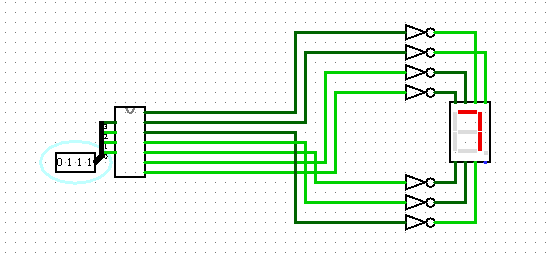
\includegraphics[width=\linewidth]{logisim_screenshots/7.png}
    \caption{Test 8}
    \label{fig:test7}
\end{figure}
Wejście (binarnie) 0111, oczekiwane wyjście (dziesiętnie) 7.\newline
Test 8 zakończony pomyślnie.

\begin{figure}[H]
    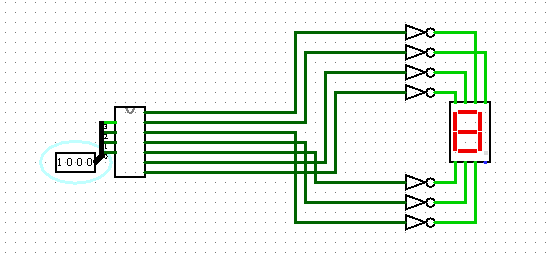
\includegraphics[width=\linewidth]{logisim_screenshots/8.png}
    \caption{Test 9}
    \label{fig:test8}
\end{figure}
Wejście (binarnie) 1000, oczekiwane wyjście (dziesiętnie) 8.\newline
Test 9 zakończony pomyślnie.

\begin{figure}[H]
    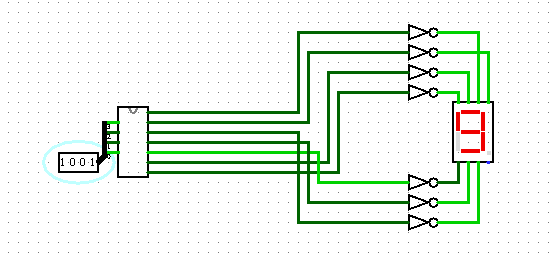
\includegraphics[width=\linewidth]{logisim_screenshots/9.png}
    \caption{Test 10}
    \label{fig:test9}
\end{figure}

Wejście (binarnie) 1001, oczekiwane wyjście (dziesiętnie) 9.\newline
Test 10 zakończony pomyślnie.

\subsection{Ocena}\label{subsec:qa-review}
Moduł 7digit.circ spełnia założenia QA.